%%%%%%%% ICML 2019 EXAMPLE LATEX SUBMISSION FILE %%%%%%%%%%%%%%%%%

\documentclass{article}

% Recommended, but optional, packages for figures and better typesetting:
\usepackage{microtype}
\usepackage{graphicx}
\usepackage{subfigure}
%\usepackage[ruled,vlined]{algorithm2e} % for pseudo code algorithm
\usepackage{booktabs} % for professional tables
\usepackage{amsmath}
\usepackage{amssymb}

% control caption space with figure
\usepackage[font=small,skip=0pt]{caption}

% hyperref makes hyperlinks in the resulting PDF.
% If your build breaks (sometimes temporarily if a hyperlink spans a page)
% please comment out the following usepackage line and replace
% \usepackage{icml2019} with \usepackage[nohyperref]{icml2019} above.
\usepackage{hyperref}

% Attempt to make hyperref and algorithmic work together better:
\newcommand{\theHalgorithm}{\arabic{algorithm}}
% adjust space
\usepackage{setspace}

% Use the following line for the initial blind version submitted for review:
\usepackage[accepted]{icml2020}

% Highlight contents with \hl{...}
\usepackage{soul}

% If accepted, instead use the following line for the camera-ready submission:
%\usepackage[accepted]{icml2019}

% The \icmltitle you define below is probably too long as a header.
% Therefore, a short form for the running title is supplied here:
\icmltitlerunning{Practical Deep Learning Approach for Intraday Futures Trading}

\begin{document}

\twocolumn[
\icmltitle{Practical Deep Learning Approach for Intraday Futures Trading}

% It is OKAY to include author information, even for blind
% submissions: the style file will automatically remove it for you
% unless you've provided the [accepted] option to the icml2019
% package.

% List of affiliations: The first argument should be a (short)
% identifier you will use later to specify author affiliations
% Academic affiliations should list Department, University, City, Region, Country
% Industry affiliations should list Company, City, Region, Country

% You can specify symbols, otherwise they are numbered in order.
% Ideally, you should not use this facility. Affiliations will be numbered
% in order of appearance and this is the preferred way.
\icmlsetsymbol{equal}{*}
\begin{icmlauthorlist}
\icmlauthor{Yuyuan Cui}{cu}
\icmlauthor{Ziyan Wang}{cu}
\end{icmlauthorlist}

\icmlaffiliation{cu}{Columbia University, New York, USA}

\icmlcorrespondingauthor{Yuyuan Cui}{yc2968@columbia.edu}
\icmlcorrespondingauthor{Ziyan Wang}{zw2569@columbia.edu}

% You may provide any keywords that you
% find helpful for describing your paper; these are used to populate
% the "keywords" metadata in the PDF but will not be shown in the document
\icmlkeywords{Deep Learning, Reinforcement Learning, Trading Strategy}

\vskip 0.3in
]

% this must go after the closing bracket ] following \twocolumn[ ...

% This command actually creates the footnote in the first column
% listing the affiliations and the copyright notice.
% The command takes one argument, which is text to display at the start of the footnote.
% The \icmlEqualContribution command is standard text for equal contribution.
% Remove it (just {}) if you do not need this facility.

%\printAffiliationsAndNotice{}  % leave blank if no need to mention equal contribution
%\printAffiliationsAndNotice{\icmlEqualContribution} % otherwise use the standard text.

\begin{abstract}
This paper provides the modeling approach and empirical results for using deep learning and reinforcement learning for developing systematic futures trading strategies in intraday timeframe. We build four deep neural network models and use them with various degrees of human experience intervention to formulate intraday futures trading strategies. By comparing prediction accuracy as well as trading performance against benchmark and across each other, we demonstrate that these models significantly outperform linear models and standard market making strategy, which supports applicability of deep learning to enhance intraday futures trading.
\end{abstract}

\section{Introduction}
\label{intro}

Deep learning has been a popular topic in quantitative financial trading. However, most studies on high frequency trading focus on developing a single type of deep learning model. Furthermore, the asset class in question is predominantly in the equities space, and features are mostly limited to order book history of the same asset traded. In this paper, we develop our intraday strategies with a more comprehensive approach. Specifically, we build two sets of independent models. The first model is an LSTM model that focuses on short-term price change prediction only. We combine the model prediction with a manually formulated simple trading strategy to make trading decisions. The second set involves three types of deep reinforcement models (double DQN, DDPG, and SAC). The action space includes buy and sell decisions and hence these models output an entire trading strategy on its own without human intervention. Moreover, we set up linear regression based models and a passive market-making strategy as benchmark. By comparing their performance, we can evaluate the applicability of deep learning in intraday futures trading with different degrees of human experience intervention. In addition, the dataset we use is China’s IH index futures tick data. This is a relatively new product that only started trading since April 2015. For feature construction, we are not constrained with order book snapshot and technical indicators, but also incorporate intraday cross-asset and time series signals that are more often seen in research on trading strategies with daily horizon. 

\section{Related Work}

Plenty of research has been done on using cross-sectional or time series data for trading on daily horizon. Xiong, Liu, Zhong, Yang and Walid (2018) used deep reinforcement learning to obtain optimal strategy based on daily return data of 30 selected stocks \cite{xiong2018practical}. Xiao Zhong and David Enke (2019) used DNNs to predict daily ETF return based on 60 financial and economic features \cite{Zhong2019}. Sezer, Ozbayoglua, and Dogdub (2017) used DNNs for optimizing technical indicators for daily stock trading and independently trained models for each of selected 30 stocks \cite{SEZER2017473}. In intraday horizon, Prakhar Ganesh and Puneet Rakheja (2018) built a standard MLP neural network for stock price prediction based on order book snapshot and reversion signal \cite{ganesh2018deep}. Svetlana Borovkova and Ioannis Tsiamas (2018) formulated stock price prediction into a classification problem and built an ensemble of LSTM networks with technical indicators as features \cite{doi:10.1002/for.2585}. Ye-Sheen Lim and Denise Gorse (2018) built Q-learning algorithm with customized CARA utility reward function and stock market order book snapshot input to optimize market making strategy \cite{DBLP:conf/esann/LimG18}. The main distinguishing features of our research are that: we compare different types of deep learning algorithms in the same setting; we perform extensive feature engineering, incorporating microstructure snapshot, technical, time series and cross-asset features as model input; we examine the less studied futures market, in particular China’s futures market.

\section{Problem Formulation}

The objective is to design deep learning models that maximize trading profit for IH futures\footnote{IH future is based on SSE 50 Index, one of the most popular index futures traded in CFFEX} based on tick-level high frequency data. We will build two types of individual models in this project. The first one is a LSTM model that focuses on short-term price movement prediction only and we manually formulate a simple trading strategy based on its predictions. The second model uses deep reinforcement learning and will output trading actions on its own. For this type, we build three individual models (double DQN, DDPG, and SAC) and will compare their performance. In addition, we will set up three benchmark trading strategies – an OLS Regression price prediction model, a Ridge Regression price prediction model, and a passive market-making strategy. By comparing our models’ performance against benchmark and against each other, we can evaluate the applicability of reinforcement learning and deep learning in intraday futures trading with various degrees of human experience intervention.

\section{Methods}

\subsection{LSTM for Mid Price Change Prediction}

The reason why we use price change as our prediction target as opposed to return is that there is no fundamental change in price scale (e.g. due to share split or drastic volatility regime shift) during the entire training and testing data sample, and that our trading horizon is constrained to be intraday. In terms of architecture, we define LSTM with 1 hidden layer, 256 hidden features, and 90 samples with 90 seconds interval. Then we process the final output of LSTM with a linear model to arrive at predicted price change. The model is trained using stochastic gradient decent algorithm with time-decaying learning rate. The price change horizon we aim to predict is simple mid change in 1 second. The LSTM architecture is illustrated in Figure \ref{fig:lstm}.

\begin{figure}[h]
	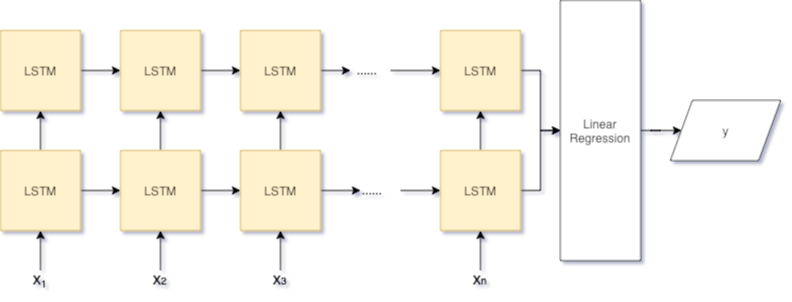
\includegraphics[width=\linewidth]{lstm.png}
	\caption{Architecture design of LSTM model for mid price prediction. Input of the model consists of 90 time series feature vectors $x_1,…,x_{90}$, sampled with 90 seconds interval. Output of the model is fed into linear regression to produce mid price change prediction. The model is trained with stochastic gradient decent algorithm.}
	\label{fig:lstm}
\end{figure}

The time series feature vector $x_t$ we use incorporates order book imbalance, cross-asset return, price-volume technical indicator, volatility and market microstructure signal such as bid-offer spread. More specifically, $x_t$ is the vector of following features as of time $t$:
\begin{itemize}
\setlength\itemsep{0.1em}
\item ${mid\_lag}_T$ ($T=1,5,10,30$): difference between current IH mid price and its mid price $T$ seconds before
\item ${wmid\_mid_T}$: snapshot difference between IH weighted mid price at $T$ and its simple mid price
\item ${wmid\_last\_price_T}$: snapshot difference beween IH weighted mid price at $T$ and its last traded price
\item ${wmid\_rolling\_min_T}$ ($T=1,5,10,30$):	difference of weighed mid of IH and its minimum in the past $T$ seconds
\item ${wmid\_rolling\_max_T}$ ($T=1,5,10,30$):	difference of weighed mid of IH and its maximum in the past $T$ seconds
\item ${trade\_dir_T}$: most recent trade direction in IH
as of time $T$
\item ${mid\_vol}_T$ ($T=30$): IH mid price volatility in the past $T$ seconds
\item ${spread}_T$ ($T=10,30,60$): IH average bid-offer spread in the past $T$ seconds
\item ${signed\_tick}_T$ ($T=10,30$): number of up price changes minus number of down price changes in the past $T$ seconds look-back interval
\item ${total\_volume}_T$ ($T=10,30$): total IH trading volume in past $T$ seconds look-back interval
\item ${signed\_volume}_T$ ($T=10, 30$): trade direction signed IH trading volume in the past $T$ seconds look-back interval
\item ${IF\_mid\_lag}_T$ ($T=5,30$): difference between current IF mid price and its mid price $T$ seconds before
\item ${IF\_mid\_vol}_T$ ($T=60$): IF mid price volatility in the past $T$ seconds
\item ${IF\_spread}_T$ ($T=10$): average IF bid-offer spread in the past $T$ seconds
\item ${IF\_total\_volume}_T$ ($T=5,30$): total IF trading volume in past $T$ seconds look-back interval
\item ${IC\_mid\_lag}_T$ ($T=5,30$): difference between current IC mid price and its mid price $T$ seconds before
\item ${IC\_mid\_vol}_T$ ($T=60$): IC mid price volatility in the past $T$ seconds
\item ${IC\_spread}_T$ ($T=10$): average IC bid-offer spread in the past $T$ seconds
\item ${IC\_total\_volume}_T$ ($T=5,30$): total IC trading volume in past $T$ seconds look-back interval
\end{itemize}

Compared with previous research that only focus on daily returns as predictive features, we take advantage of the most granular level of tick-by-tick data (with average update frequency of less than one second), which provide a much larger dataset for training complex deep learning models. Compared with previous high-frequency trading research that mostly used either order book snapshot or time series signal for each individual asset, we construct a much wider range of features that encompass information in order book imbalance, trading volume, trading direction, technical time series pattern, and cross-asset returns. The reason why we choose not to include cross-asset trade or book information is because based on out-sample testing, the additional predictive power to that already included in cross-asset price change is not meaningful and hence we prefer a simpler model for robustness consideration.

\subsection{Deep Reinforcement Learning for Intraday Trading}

The financial trading setting can be formulated as a reinforcement learning problem. The state of the agent is the amount of position it’s holding, together with market condition variables $x_t$ described in the LSTM model section. The immediate reward is just the “one-step” (2 seconds) return of its current portfolio holding, and the action space is the buy/sell decisions. As there is no ambiguity in return calculation and state transition from historical tick data, we focus our modeling effort on the optimal policy learning as opposed to modeling environment dynamics for planning. Therefore, we choose the model-free type of reinforcement learning. In the following sections, we examine three popular deep reinforcement algorithms: Q-learning based DQN, and policy optimization algorithms DDPG and SAC.

\subsubsection{Double Deep Q Learning (DQN)}

\begin{figure}[h]
	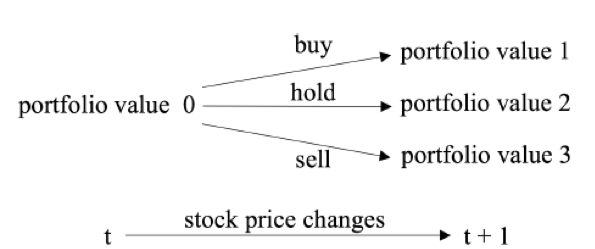
\includegraphics[width=\linewidth]{rl_strat.png}
	\caption{We've defined three actions for Q-learning: buy, hold and sell.}
	\label{fig:rl_strat}
\end{figure}

To characterize the state space, we will use the same features in the LSTM model for comparison purpose. In addition, we add current futures position holding as feature describing the environment. For simplicity, we restrict actions to be either long one additional contract, short one additional contract or no change in position held. As a result, the DNN’s output should be three-dimensional to reflect estimate of value of these three actions. We model the Q function through a DNN with two hidden layers (each has a dimension of 10 and with ReLu activation). Furthermore, to facilitate calibration, we use market value of position holding 1 minute since initial setting up a position as “terminal state”. Due to high degree of noise commonly seen in financial data, we choose a Double Q-learning approach to improve robustness and alleviate the risk of overestimating action values. Specifically, we will use the iterative approach (see Figure \ref{fig:rl_loop} and Algorithm \ref{alg:dqn}) to update the two DNN-based $Q(\mathbf{s}_t, \mathbf{a}_t)$ function estimates, with a cyclic buffer for memory replay. The neural network parameters are optimized using the Adam algorithm.
\begin{figure}[h]
	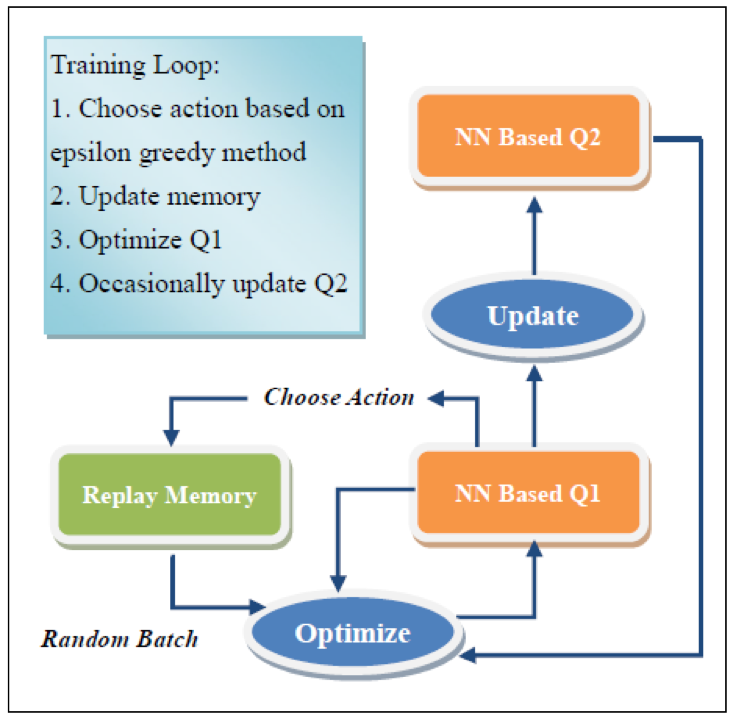
\includegraphics[width=\linewidth]{rl_loop.png}
	\caption{The training loop for the double DQN model for mid price prediction}
	\label{fig:rl_loop}
\end{figure}

\begin{algorithm}[h]
	\caption{Double DQN algorithm}
	\label{alg:dqn}
	\begin{algorithmic}
		\setstretch{0.6}
		\STATE Input: $\mathcal{D}$ - empty replay buffer; $\theta$ - initial network parameters, $\theta^-$ - copy of $\theta$
		\STATE Input: $N_r$ - replay buffer maximum size; $N_b$ - training batch size; $N^-$ - target network replacement freq.
		\FOR{$episode e \in \{1,2,...,M\}$}
			\STATE Initialize frame sequence $\mathbf{x}\leftarrow()$
			\FOR{$t\in\{0,1,...\}$}
				\STATE Set $\mathbf{s} \leftarrow \mathbf{x}$, sample action $\mathbf{a}\sim\pi_{\mathcal{B}}$
				\STATE Sample next frame $x^t$ from environment $\mathcal{E}$ given $(\mathbf{s}, \mathbf{a})$ and receive reward $r$, and append $x^t$ to $\mathbf{x}$
				\IF{$ |\mathbf{x}| > N_f $}
					\STATE Delete oldest frame $x_{t_{min}}$ from $\mathbf{x}$ end
				\ENDIF
				\STATE Set $\mathbf{s'} \leftarrow \mathbf{x}$, and add transition tuple $( \mathbf{a},\mathbf{a}, r, \mathbf{s'})$ to $\mathcal{D}$, replacing the oldest tuple if $|\mathcal{D}| \geq N_r$
				\STATE Sample a minibatch of $N_b$ tuples $( \mathbf{a},\mathbf{a}, r, \mathbf{s'}) \sim \mathrm{Unif} (\mathcal{D})$
				\STATE Construct target values, one for each of the $N_b$ tuples:
				\STATE Define $\mathbf{a}^{\max}( \mathbf{s'; \mathbf{\theta}} = \mathrm{arg} \max_{\mathbf{a'}} Q(\mathbf{s'}, \mathbf{a'}; \mathbf{\theta}) )$
				\[
					y_j = \begin{cases}
					\mbox{$r$,} & \mbox{if } s' $is terminal$ \\
					\mbox{$r + \gamma Q( \mathbf{s'}, \mathbf{a}^{\max} ( \mathbf{s'} ; \mathbf{\theta} ); \mathbf{\theta^-} )$} & \mbox{otherwise}
					\end{cases}
				\]
				\STATE Do a gradient descent step with loss ${ || y_j - Q ( \mathbf{s}, \mathbf{a}; \mathbf{\theta} ) || }^2$
				\STATE Replace target parameters $\theta^- \leftarrow \theta \mathrm{every} N^- \mathrm{steps}$
			\ENDFOR
		\ENDFOR
	\end{algorithmic}
\end{algorithm}

\subsubsection{Deep Deterministic Policy Gradient (DDPG)}

A key limitation for the DQN framework is its discrete nature of action space. However, given the size of our trading order is variable, it is reasonable to model action as a continuous variable. 

\begin{figure}[h]
	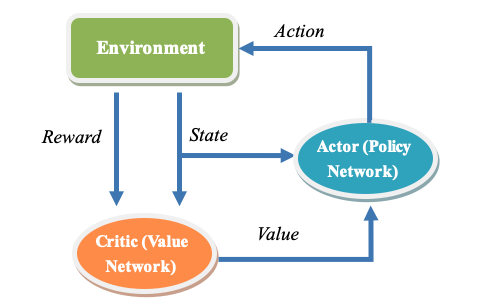
\includegraphics[width=\linewidth]{ddpg_flow1.png}
	\caption{We train the DDPG model using Actor-Critic method where the Critic is used to approximate Q value function for a given state-action pair and is a deep neural network, and the Actor is used to approximate optimal policy deterministically.}
	\label{fig:ddpg_flow1}
\end{figure}

In contrast to DQN that finds optimal policy by looking up an estimated Q function, DDPG uses a DNN to directly return a single optimal action given an input state. We train the DDPG model using Actor-Critic method. The Actor is used to approximate optimal policy deterministically and is a DNN with 2 hidden layers (with dimension of 40 and 30, respectively), with ReLu activation for hidden layers and tanh for output layer. To facilitate exploration, we add an Ornstein-Ulhenbeck noise to the action produced by Actor.
$$\mu'(\mathbf{s}_t) = \mu( \mathbf{s}_t | \theta^\mu_t) + \mathcal{N}$$
The Actor network is trained using sampled policy gradient:
\begin{align*}
& J(\theta) = \mathbb{E} [Q (\mathbf{s},\mathbf{a}) | \mathbf{s}=\mathbf{s}_t, \mathbf{a}_t=\mu(\mathbf{s}_t)] \\
& \nabla_{\theta^\mu}J(\theta) \approx \nabla_a Q(\mathbf{s},\mathbf{a}) \nabla_{\theta^\mu} \mu(\mathbf{s}|\theta^\mu) \\
& \nabla_{\theta^\mu}J \approx \frac{1}{N} \sum_{i} [ \nabla_a Q(\mathbf{s},\mathbf{a} | \theta^Q) |_{\mathbf{s}=\mathbf{s}_i, \mathbf{a}=\mu(\mathbf{s}_i)} \nabla_{\theta^\mu} \mu(\mathbf{s} | \theta^\mu)|_{\mathbf{s}=\mathbf{s}_i} ]
\end{align*}
The Critic is used to approximate Q value function for a given state-action pair and is a DNN with 3 hidden layers (with dimensions of 40, 30, and 10 respectively), with ReLu activation for hidden layers and linear function for output layer. The value function is trained using the temporal difference estimate.
\begin{align*}
Q^{Actual} ( \mathbf{s}_t, \mathbf{a}_t ) & = r ( \mathbf{s}_t, \mathbf{a}_t ) + \gamma Q' ( \mathbf{s}_{t+1}, \mathbf{\mu}' ( \mathbf{s}_{t+1} | \mathbf{\theta}^{\mathbf{\mu'}} ) | \mathbf{\theta}^{Q'}  )\\
Loss(\mathbf{\theta}^Q ) & = \frac{1}{N} \sum_{i} ( Q^{Actual} ( \mathbf{s}_i, \mathbf{a}_i ) - Q ( \mathbf{s}_i, \mathbf{a}_i | \mathbf{\theta}^{Q} ) )^2
\end{align*}
To improve training stability, we keep a target network for Actor (denoted as $Q'$) and a target network for Critic (denoted as $\mu'$). While the “regular” Actor and Critic networks are updated during the experience replay stage, the “target” networks are only updated occasionally, using a soft update strategy:
$$\theta^{Q'} \leftarrow \tau\theta^Q + (1-\tau)\theta^{Q'} $$
$$\theta^{\mu'} \leftarrow \tau\theta^\mu + (1-\tau)\theta^{\mu'} $$

The pesudocode is shown in Algorithm \ref{alg:ddpg} and the algorithm flow chart is shown in Figure \ref{fig:ddpg_flow}.
\begin{figure}[h]
	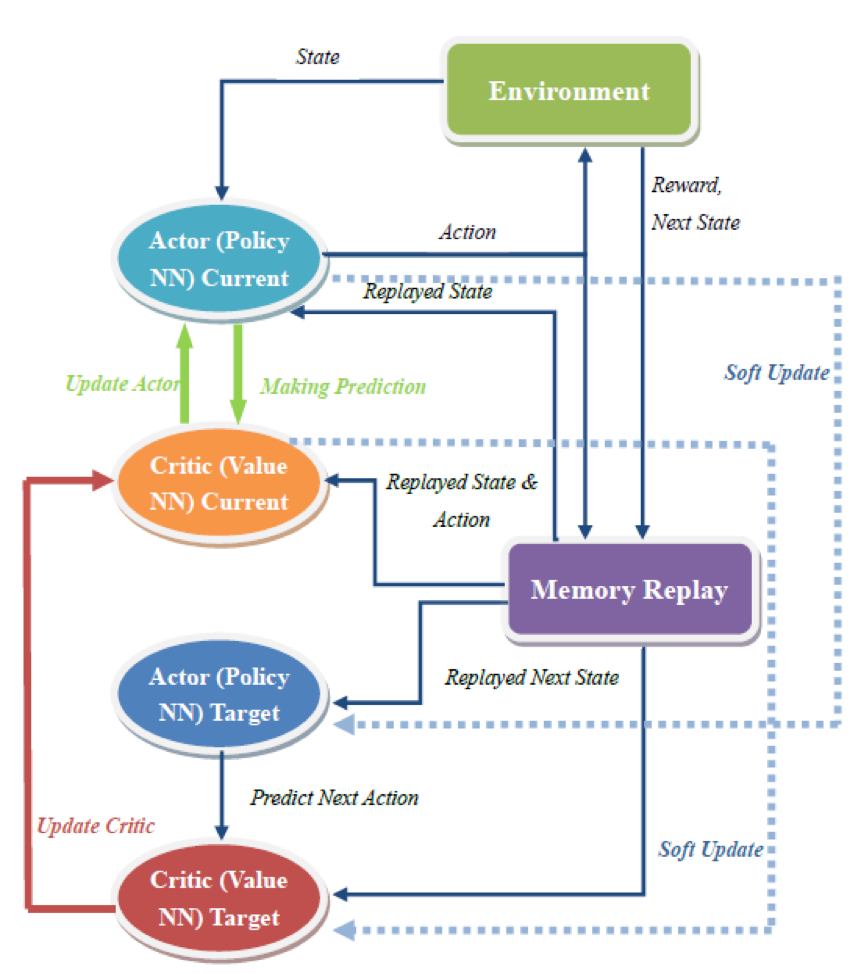
\includegraphics[width=\linewidth]{ddpg_flow.png}
	\caption{General overview of DDPG algorithm flow}
	\label{fig:ddpg_flow}
\end{figure}

\begin{algorithm}[h]
	\caption{DDPG algorithm}
	\label{alg:ddpg}
	\begin{algorithmic}
		\setstretch{0.6}
		\STATE Randomly initialize critic network $Q(s,a|\theta^Q)$ and actor $\mu(s|\theta^\mu)$ with random weight $\theta^Q$ and $\theta^\mu$;
		\STATE Initialize replay buffer $R$;
		\FOR{$episode=1$, $M$}
			\STATE Initialize a random process $N$ for action exploration;
			\STATE Receive initial observation state $s_1$;
			\FOR{$t=1, T$}
				\STATE Select action $a_t=\mu(s_t|\theta^\mu) + N_t$ according to the current policy and exploration noise;
				\STATE Execute action $a_t$ and observe reward $r_t$ and state $s_{t+1}$;
				\STATE Store transition $(s_t, a_t, r_t, s_{t+1})$ in $R$;
				\STATE Sample a random minibatch of $N$ transitions $(s_i , a_i , r_i , s_{i+1})$ from $R$;
				\STATE Set $y_i = r_i + \gamma Q'(s_{t+1}, \mu'(s_{i+1} | \theta^{\mu'} | \theta^{Q'} ))$;
				\STATE Update critic by minimizing the loss:$$L = \frac{1}{N} \sum_{i} {(y_i-Q(s_i, a_i | \theta^Q))}^2$$
				\STATE Update the actor policy by using the sampled policy gradient:
				\begin{multline*}
				\nabla_{\theta^\mu}J\approx\frac{1}{N}\sum_{1} \nabla_a Q(s,a|\theta^Q) |_{s=s_i, a=\mu(s_i)}\\
				\times \nabla_{\theta^\mu} \mu(s|\theta^\mu)|_{s_i}
				\end{multline*}
				\STATE Update the target networks:
				$$\theta^{Q'} \leftarrow \tau\theta^Q + (1-\tau)\theta^{Q'} $$
				$$\theta^{\mu'} \leftarrow \tau\theta^\mu + (1-\tau)\theta^{\mu'} $$
			\ENDFOR
		\ENDFOR
	\end{algorithmic}
\end{algorithm}

\subsubsection{Soft Actor-Critic (SAC)}

Another deep reinforcement model for continuous action space is the SAC model, which also considers maximizing the entropy of the policy, thus encouraging exploration and assign similar probabilities to actions with equal Q-values.
$$J(\pi) = \sum_{t=0}^{T} \mathbb{E}_{(\mathbf{s}_t, \mathbf{a}_t)\sim\rho_\pi} [r(\mathbf{s}_t, \mathbf{a}_t)+\alpha \mathcal{H} (\pi( \cdot | \mathbf{s}_t))]$$
where $H$ is the entropy of policy distribution. The entropy of any continuous random variable $X$ with probability
density function $p$ is defined as:
$$\mathcal{H}(X)=-\int_{-\infty}^{\infty} p(x)\log p(x)dx$$

We set up our SAC model with three deep neural networks: 

1) a state value function V
\begin{equation*}
\label{eq1}
\begin{split}
V^\pi(\mathbf{s}) & =  \underset{( \mathbf{s}_t, \mathbf{a}_t ) \sim \rho_\pi}{\mathbb{E}} \bigg[ \sum_{t=0}^{T} \gamma^t (r(\mathbf{s}_t,\mathbf{a}_t)\\
& + \alpha \mathcal{H} ( \pi ( \cdot | \mathbf{s}_t) ) ) | \mathbf{s}_0=\mathbf{s} \bigg] \\
& = \underset{\mathbf{a} \sim \rho_\pi}{\mathbb{E}} [ Q^\pi (\mathbf{s},\mathbf{a}) ] + \alpha \mathcal{H} ( \pi( \cdot | \mathbf{s}) ) \\
& = \underset{\mathbf{a} \sim \rho_\pi}{\mathbb{E}} [Q^\pi(\mathbf{s},\mathbf{a}) - \alpha \log \pi ( \mathbf{a} | \mathbf{s}) ]\\
& \approx Q^\pi (\mathbf{s}, \tilde{\mathbf{a}} ) - \alpha \log \pi ( \tilde{\mathbf{a}} | \mathbf{s}),\: \tilde{\mathbf{a}} \sim \pi( \cdot | \mathbf{s})
\end{split}
\end{equation*}
2) a Q-function
\begin{equation*}
\label{eq2}
\begin{split}
& Q^\pi ( \mathbf{s},\mathbf{a} ) \\
& =  \underset{( \mathbf{s}_t, \mathbf{a}_t ) \sim \rho_\pi}{\mathbb{E}} \bigg[ \sum_{t=0}^{T} \gamma^t r (\mathbf{s}_t,\mathbf{a}_t)\\
& + \alpha \sum_{t=1}^{T} \gamma^t \mathcal{H} ( \pi ( \cdot | \mathbf{s}_t) ) ) | \mathbf{s}_0 = \mathbf{s}, \mathbf{a}_0 = \mathbf{a} \bigg] \\
& = \underset{( \mathbf{s}', \mathbf{a}' ) \sim \rho_\pi}{\mathbb{E}} [ r (\mathbf{s},\mathbf{a}) + \gamma ( Q^\pi ( \mathbf{s}', \mathbf{a}' ) + \alpha \mathcal{H} ( \pi ( \cdot | \mathbf{s}' )))] \\
& = \underset{( \mathbf{s}') \sim \rho_\pi}{\mathbb{E}} [ r(\mathbf{s},\mathbf{a}) + \gamma V^\pi (\mathbf{s}') ]
\end{split}
\end{equation*}
To prevent overestimation, we use two Q networks and take the minimum value of them for both the policy and value function updates. The architecture of the two Q networks are the same - 2 hidden layers (both of dimension 30) with ReLu activation. Output activation is linear.

3) a policy function $\pi$
$$\pi ( \mathbf{a}_t | \mathbf{s}_t ) \sim \mathcal{N} \bigg( f_{\mathrm{neural\:network}} ( \mathbf{s}_t); \sum \bigg)$$
Policy is modeled through a Gaussian distribution with mean computed from a DNN that has 2 hidden layers (both have dimension 30) with ReLu activation. Output activation is linear.

We train the Q function network based on mean squared Bellman error (MSBE). To improve stability, we introduce a target network for the value function which is fixed when updating Q function. The Q function is updated using Adam algorithm.
\begin{equation*}
\begin{split}
	L(\phi_i,\mathcal{D}) & = \underset{(\mathbf{s}_t, \mathbf{a}_T) \sim \mathcal{D}}{\mathbb{E}} [ { (Q_{\phi_i} (\mathbf{s}_t, \mathbf{a}_t) - \hat{Q_1} ( \mathbf{s}_t, \mathbf{a}_t ))}^2 ]\\
	& = \underset{(\mathbf{s}_t, \mathbf{a}_T) \sim \mathcal{D}}{\mathbb{E}} [  (Q_{\phi_i} (\mathbf{s}_t, \mathbf{a}_t) - r(\mathbf{s}_t, \mathbf{a}_t)\\
	& - \gamma \underset{\mathbf{s}_{t+1}}{\mathbb{E}} [ V_{\psi_{targ}} ( \mathbf{s}_{t+1} ) ] )^2 ] \\
\end{split}
\end{equation*}
We train the value network based on mean-squared-error loss between current and entropy-adjusted Q value, where we use clipped double-Q form that takes the minimum of the two approximation networks. The value function is updated using Adam algorithm.
\begin{equation*}
\begin{split}
L(\psi,\mathcal{D}) & = \underset{\mathbf{a}_t\sim\pi_\theta}{\underset{\mathbf{s}_t\sim\mathcal{D}}{\mathbb{E}}}  \Big[ (V_\psi(\mathbf{s}_t) - (\min_{i=1,2} Q_{\phi_i}(\mathbf{s}_t, \tilde{\mathbf{a}}) \\
& - \alpha \log\pi_\theta( \tilde{\mathbf{a}} | \mathbf{s}_t)))^2 \Big], \: \tilde{\mathbf{a}} \sim \pi( \cdot | \mathbf{s}) \\
\end{split}
\end{equation*}
We train the policy network using the reparameterization trick. This process ensures that sampling from the policy is a differentiable process. 
$$\tilde{a}(\mathbf{s}_t, \xi_t) = \mathrm{tanh} (\mu(\mathbf{s}_t) + \sigma(\mathbf{s}_t) \odot \xi_t),\: \xi_t \sim \mathcal{N}(0, I)$$
Using the first of the two Q networks as approximation for Q value, we have the optimization re-stated as the following form:
\begin{equation*}
\begin{split}
J(\theta) & = \max_{\theta} \underset{\mathbf{\xi}_t \sim \mathcal{N}}{\underset{\mathbf{s}_t\sim\mathcal{D}}{\mathbb{E}}}  
[ Q_{\phi_1} (\mathbf{s}_t, \tilde{\mathbf{a}} (\mathbf{s}_t, \xi_t))\\
& - \alpha \log \pi ( \tilde{\mathbf{a}} (\mathbf{s}_t, \xi_t) | \mathbf{s}_t)))^2]
\end{split}
\end{equation*}

We will update policy network with Adam algorithm.

The pseudocode for the SAC algorithm is given in Algorithm \ref{alg:sac}.

\begin{algorithm}[h]
	\caption{Soft Actor-Critic}
	\label{alg:sac}
	\begin{algorithmic}
		\setstretch{0.1}
		\STATE Inital policy parameters $\theta$, Q-function parameters $\phi_1$, $\phi_2$, V-function parameters $\psi$, empty replay buffer $\mathrm{D}$
		\REPEAT
			\STATE Observe state s and select action $a\sim\pi_\theta(\cdot|s)$
			\STATE Execute $a$ in the environment
			\STATE Observe next state $s'$, reward $r$, and done signal $d$ to indicate whether $s'$ is terminal
			\STATE Store $(s,a,r,s',d)$ in replay buffer $\mathrm{D}$
			\IF {$s'$ is terminal}
			\STATE  reset environment state 
			\ENDIF
			\IF {If it's time to update}
				\FOR{$j$ in range (however many updates)}
					\STATE Randomly sample a batch of transitions, \\
					$B=(s,a,r,s',d)$ from $\mathrm{D}$
					\STATE Compute targets for $Q$ and $V$ functions:
					\STATE 
					\begin{align*} 
					y_q (r,s',d) &=  r+\gamma(1-d)V_{\psi_{targ}}(s') \\ 
					y_v(s) &= \min_{i=1,2} Q_{\psi_i}(s,\bar{a}) - \alpha\log\pi_\theta(\bar{a}|s), \\
					& \bar{a}\sim\pi_\theta(\cdot|s)
					\end{align*}
					\STATE Update Q-functions by one step of gradient descent using
					$$\nabla_{\phi_i} \frac{1}{|B|} \sum_{(s,a,r,s',d)\in B} {(Q_{\phi,i}(s,a) - y_q(r,s',d))}^2$$
					$\mathrm{for}$  $i=1,2$
					\STATE Update V-function by one step of gradient descent using
					$$\nabla_{\psi} \frac{1}{|B|} \sum_{s\in B} {(V_{\psi}(s) - y_v(s))}^2$$
					\STATE Update policy by one step of gradient ascent using
					$$\nabla_{\theta} \frac{1}{|B|} \sum_{s\in B} {(Q_{\phi,1}(s,\tilde{a}_\theta)\alpha\log\pi_\theta(\tilde{a}_\theta(s)|s)}$$
					where $\tilde{a}_\theta(s)$ is a sample from $\pi_\theta(\cdot|s)$ which is a differentiable wrt $\theta$ via the reparametrization trick
					\STATE Update target value network with
					$$\psi_{targ}\leftarrow\rho\psi_{targ}+(1-\rho)\psi$$
				\ENDFOR
			\ENDIF
		\UNTIL{convergence}
	\end{algorithmic}
\end{algorithm}

\section{Results}

\subsection{Data}

The dataset we use is tick data of IH futures (SSE 50 Stock Index Futures), IC futures (CSI 500 Stock Index Futures) and IF (CSI 300 Stock Index Futures) futures tick data in China’s CFFEX exchange in 2018. The data include all book updates and trade events. The morning trading session is 09:30 AM - 11:30 AM and the after session is 01:00 PM – 03:00 PM. We treat data in any look-back period outside of session (e.g. 9:20 AM or 12:30 PM) as NaN but otherwise treat both sessions equally. For each futures, we use front-month contract (contract that expires in the next month). As maximum tick frequency is around 0.5 seconds, we regularize all data with resample frequency of 0.5 seconds. For missing data, we fill last traded price, bid/offer price and size with most recent valid value; and fill traded volume with 0. In back-testing, we always close all positions whenever a trading session ends. The model training (in-sample) period is 1/1/2018 to 8/31/2018, validation period is 9/1/2018 to 9/30/2018 and the testing (out-sample) period is 10/1/2018 to 12/31/2018.

\subsection{Model Performance}

\subsubsection{LSTM for Mid Price Change Prediction}

We evaluate the LSTM model using mean-squared error (MSE) of predicted compared with actual mid price change. Model performance is compared with OLS and Ridge Regression using same set of features as benchmark. Table \ref{tab:mse} shows that LSTM has significantly lower MSE and the generalization error (measured by increase from in-sample to out-sample MSE) is also lower. Therefore, from fitting perspective, the predictive power of LSTM is better and more robust than standard linear models.
\begin{table}[h]
	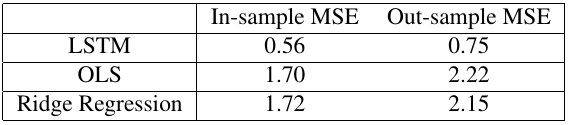
\includegraphics[width=\linewidth]{mse.png}
	\caption{Performance comparison between our LSTM model and ridge regression model and OLS model} 
	\label{tab:mse}
\end{table}

Next, we examine its performance through two-way table. As Table \ref{tab:tw_in} and Table \ref{tab:tw_out} show, in a predominant portion of sample, the short-term mid change is smaller than one tick (a full bid-ask spread), which means that even with perfect predictive modeling, we may still not be able to trade profitably after accounting for the transaction cost of crossing the bid-ask spread. A good trading signal should capture market moves that are more than one tick and avoid taking unnecessary positions that won’t realize gains in excess of transaction cost. LSTM achieves this objective better than linear models. In Table \ref{tab:tw_out}, in out-sample trading, LSTM makes less error in taking a position bet that turns out to be a move within a tick and makes more correct bet when the market actually moves more than a tick. In contrast, linear models make more conservative or wrong prediction when market actually makes major move.
\begin{table}[h]
	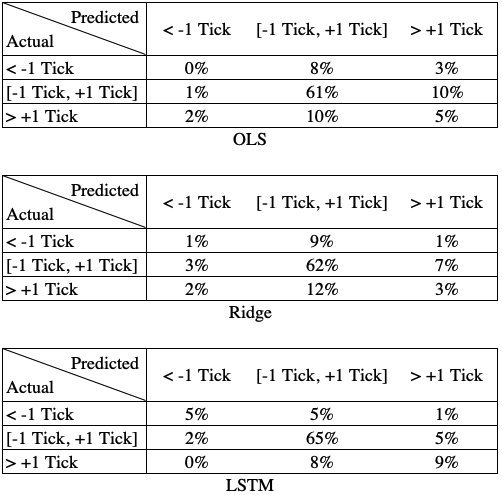
\includegraphics[width=\linewidth]{tw_in_sample.png}
	\caption{Two-way table of in-sample training} 
	\label{tab:tw_in}
\end{table}
\begin{table}[h]
	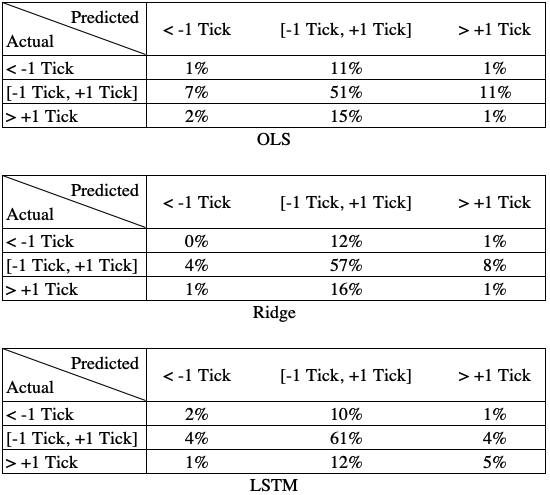
\includegraphics[width=\linewidth]{tw_out_sample.png}
	\caption{Two-way table of out-sample testing} 
	\label{tab:tw_out}
\end{table}
Next, we compare the performance of a simple trading strategy guided by the LSTM with the benchmark. The LSTM-based strategy buys when it predicts the price will move up by at least 0.25, places sells when it predicts the price will move down by at least 0.25, and takes no action otherwise. The benchmark strategy, however, always places both a bid and an offer order. We restrict both strategies to hold a maximum of three contracts. As Figure \ref{fig:bt_pnl} shows, the LSTM model outperforms the benchmark strategy while linear models have a hard time making profits.

\subsubsection{Deep Reinforcement Learning for Intraday Trading}

Figure \ref{fig:perf_compare} shows the average of total rewards in the rolling 10 epochs of training. All three reinforcement learning models achieves a stable level within 1,000 epochs.
\begin{figure}[h]
	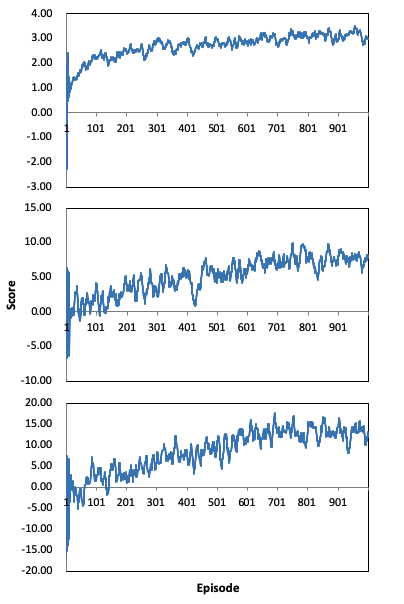
\includegraphics[width=\linewidth]{in_sample_perf_compare.png}
	\caption{Comparison of in-sample learning performance (measured by moving average of returns over most recent 10 epochs of training) for the three deep RL models. From top to bottom are for DQN, DDPG and SAC respectively. Out-sample backtesting period is 10/01/2018 – 12/31/2018}
	\label{fig:perf_compare}
\end{figure}
\begin{table}[h]
	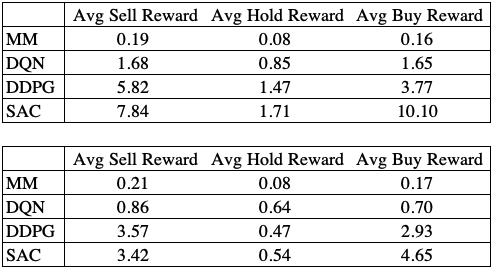
\includegraphics[width=\linewidth]{rl_avg_perf.png}
	\caption{Comparison of average rewards of buy, hold and sell actions for three reinforcement algorithms: DQN, DDPG and SAC, and a market making strategy}
	\label{tab:rl_avg_perf}
\end{table}
To better evaluate them in a trading strategy setup, we look at average immediate reward of taking an action, which is measured as one-step (2 seconds) return of position holding after taking action. All three models outperform the benchmark strategy. Furthermore, DDPG and SAC has higher rewards in the “Buy” and “Sell” action columns. This is because their action space is continuous and that allows the models to bet more aggressively in times of greater confidence.

\subsubsection{Trading Performance Comparison}
\begin{figure}[h]
	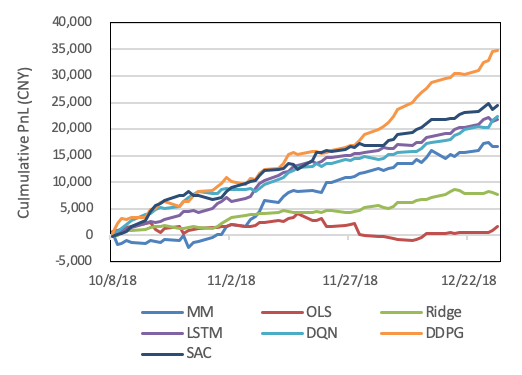
\includegraphics[width=\linewidth]{bt_res.png}
	\caption{Comparison of cumulative trading PnL for each of the 7 trading strategies (strategies based on OLS, Ridge, LSTM, DQN, DDPG, SAC, and the benchmark market making strategy) over the out-sample backtesting period (10/01/2018 – 12/31/2018)}
	\label{fig:bt_pnl}
\end{figure}
\begin{table}[h]
	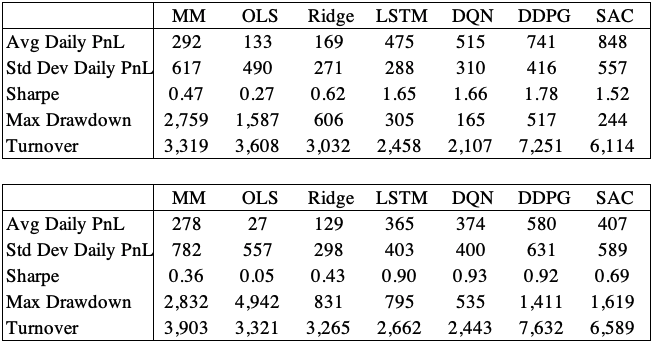
\includegraphics[width=\linewidth]{perf_stats.png}
	\caption{Trading performance statistics for for each of the 7 trading strategies (strategies based on OLS, Ridge, LSTM, DQN, DDPG, SAC, and the benchmark market making strategy). In-sample data is shown in the upper table while out-sample data is shown in the lower table. In-sample period is 01/01/2018 – 8/31/2018, and out-sample period is 10/01/2018 – 12/31/2018}
	\label{tab:perf_stats}
\end{table}
We put the cumulative profit-and-loss (pnl) plot for all of the models together for out-sample backtesting in Figure \ref{fig:bt_pnl}. In addition, we calculate trading performance statistics for these models in Table \ref{tab:perf_stats}. In terms of overall return, DDPG is the best, followed by SAC. This shows that the flexibility of position sizing in these algorithms brings greater return potential. However, it does not appear entropy regularization in SAC results in meaningful improvement from DDPG. In terms of risk profile, LSTM and DQN have a lower Sharpe but also lower drawdown and volatility. This makes them more suitable for risk-averse investors. The four deep learning models all beat the benchmark strategies.

\subsection{Analysis}

The LSTM model has greater flexibility in capturing both the sequential dependency and complex inter-feature interaction of the high dimensional feature time series. As a result, both in-sample and out-sample MSE are significantly lower than OLS and Ridge. The model-based strategy also outperforms passive (uninformed) trading strategy. The benchmark strategy trades more frequently and often suffers from adverse selection. In comparison, both the LSTM model and the three RL models are more cautious in entering into positions and only trade when they have confidence in predicted direction. Extending LSTM model with human input to end-to-end deep reinforcement learning (DQN, DDPG, and SAC), we achieve even higher return This means that we can delegate both price prediction and position management to deep learning models. 

\subsection{Project Repository}
\href{https://github.com/louiswang01/deep-learning-for-futures-trading}{https://github.com/louiswang01/deep-learning-for-futures-trading}

% In the unusual situation where you want a paper to appear in the
% references without citing it in the main text, use \nocite
%\pagebreak
\bibliographystyle{icml2020}
\bibliography{final}


\end{document}


% This document was modified from the file originally made available by
% Pat Langley and Andrea Danyluk for ICML-2K. This version was created
% by Iain Murray in 2018, and modified by Alexandre Bouchard in
% 2019. Previous contributors include Dan Roy, Lise Getoor and Tobias
% Scheffer, which was slightly modified from the 2010 version by
% Thorsten Joachims & Johannes Fuernkranz, slightly modified from the
% 2009 version by Kiri Wagstaff and Sam Roweis's 2008 version, which is
% slightly modified from Prasad Tadepalli's 2007 version which is a
% lightly changed version of the previous year's version by Andrew
% Moore, which was in turn edited from those of Kristian Kersting and
% Codrina Lauth. Alex Smola contributed to the algorithmic style files.
